%===================================== CHAP 5 =================================

\chapter{Implementation}
\label{chp:implementation}

\figurename~\ref{fig:architecture-overview} shows a high level overview of the
CARP hardware platform extended with a readout module. While the system has been
extended with new functionality and partially ported to Chisel, the overall
architecture of the system has been largely preserved. In
\figurename~\ref{fig:architecture-detail}, a more detailed view of the system is
shown. Modules are annotated with either a C(hisel) or a V(HDL) in the upper
right corner to indicate their porting status. The top level logic and wiring
gluing all the modules together is all done in Chisel.

\begin{figure}[ht]
  \centering
  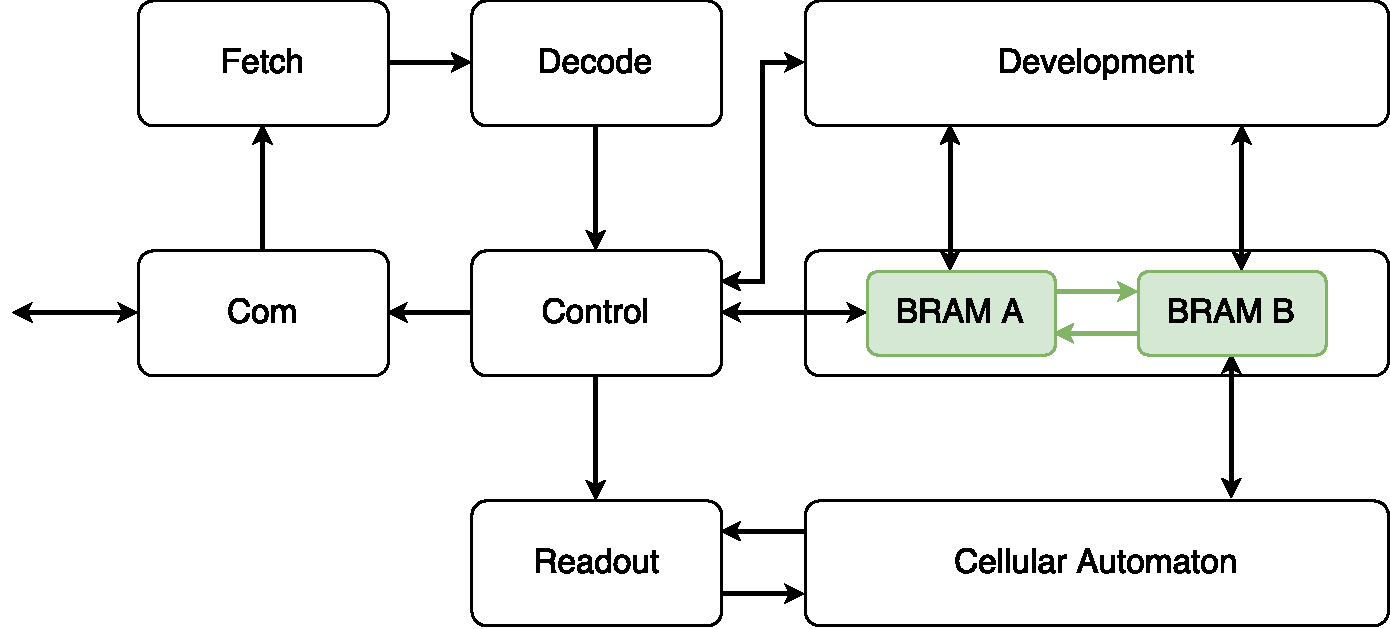
\includegraphics[width=0.8\linewidth]{fig/architecture-overview}
  \caption{
    Block diagram of the CARP hardware architecture extended with a readout layer.
  }
  \label{fig:architecture-overview}
\end{figure}

\begin{sidewaysfigure}[ht]
    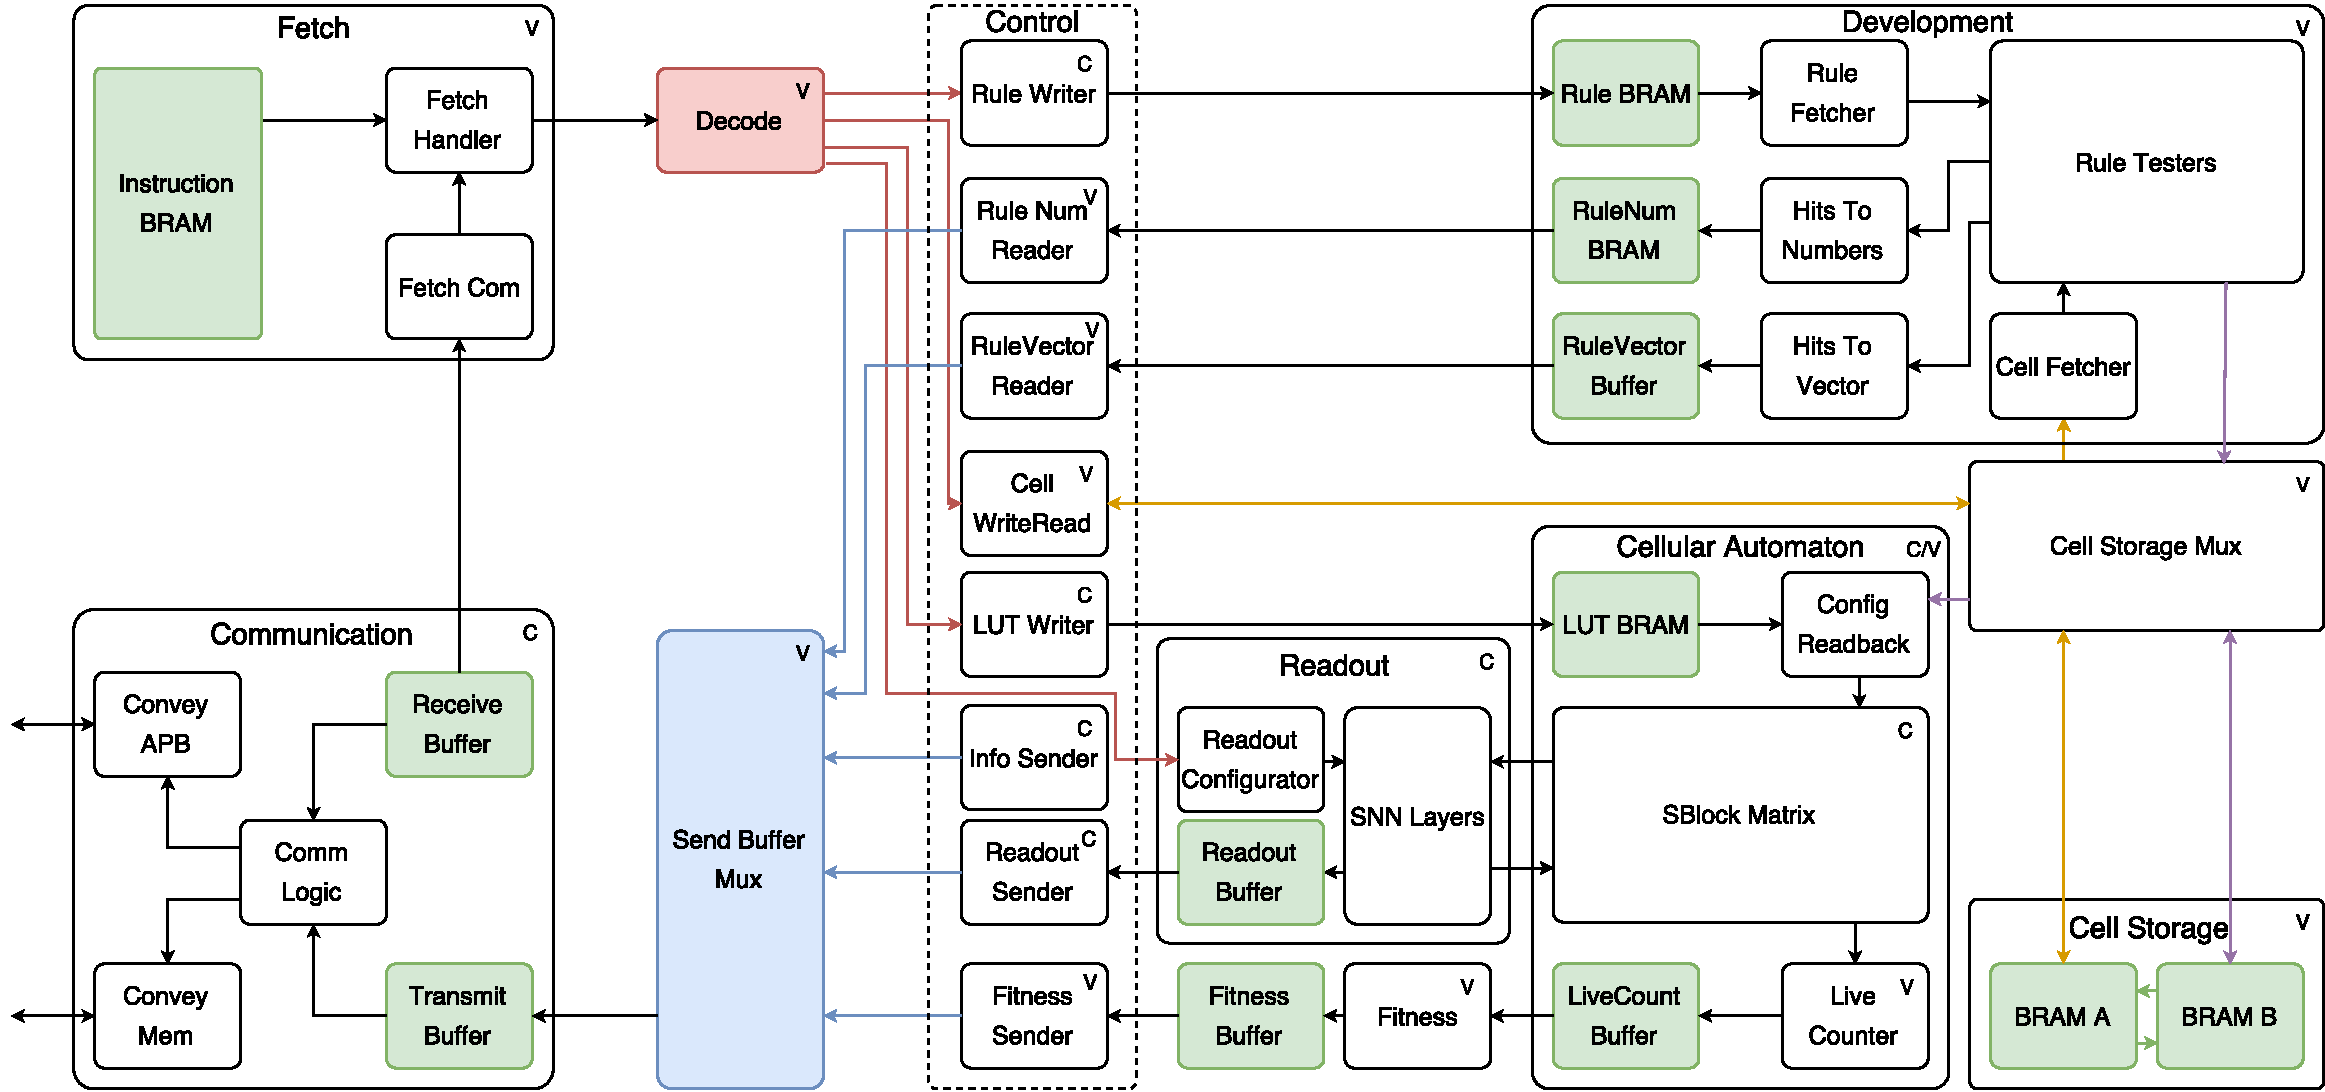
\includegraphics[width=\textwidth]{fig/architecture-detail}
    \caption{
      Modified reprint from~\cite{Lundal2015a} showing a detailed overview of
      the CARP architecture and its constituent modules. Modules annotated with a C in
      the upper right corner are implemented in / have been ported to Chisel, while
      those annotated with a V are implemented in VHDL. Child modules not annotated
      are implemented in the same language as their parent modules. Signals indicate
      flow of data or direction of communication, control signals and detailed
      interfaces are ommited for clarity.
    }
    \label{fig:architecture-detail}
\end{sidewaysfigure}
\clearpage

\section{General overview}


\clearpage

\section{Communication}
\label{sec:communication}

As outlined in section~\ref{sec:coproc}, the FPGA on the Convey coprocessor is
logically divided into Application Engines within which any custom logic can be
implemented. Each AE can communicate with the host, the on-board memory and
other AEs through various interfaces implemented by the Convey PDK, shown in
\figurename~\ref{fig:convey-ae-io-overview}. To be able to run the CARP hardware
platform on the coprocessor, the communication module has been reimplemented to
utilize these interfaces for data transfer.

\begin{figure}[ht]
  \centering
  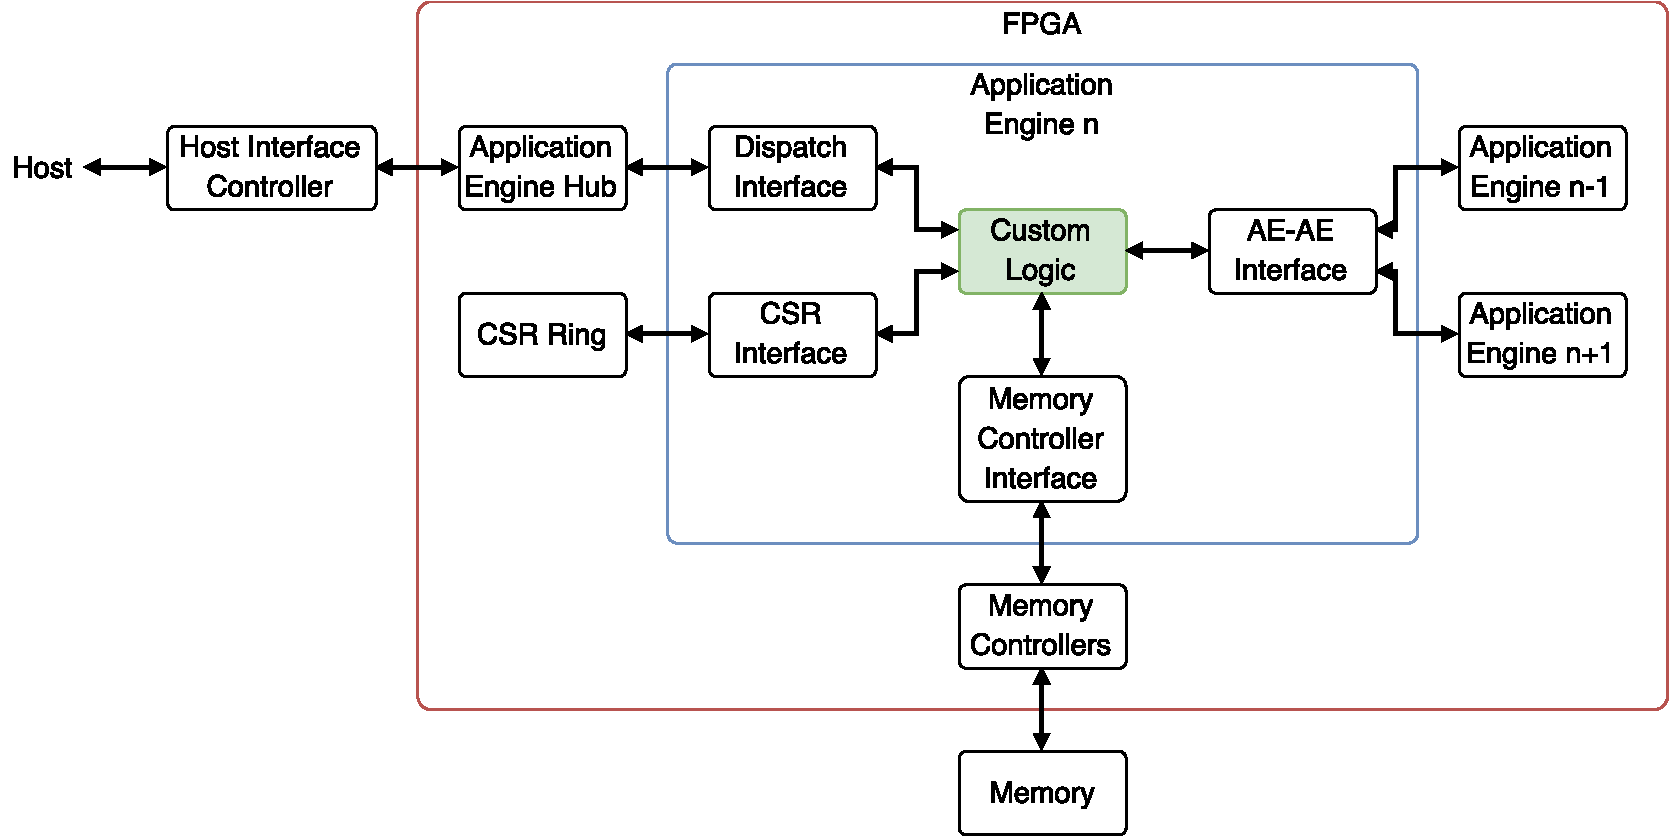
\includegraphics[width=\linewidth]{fig/convey-ae-io-overview}
  \caption{Overview of the Convey Application Engine architecture.}
  \label{fig:convey-ae-io-overview}
\end{figure}

\figurename~\ref{fig:convey-io-carp-overivew} shows how the CARP hardware is
implemented within the Convey AE architecture. The communication module has been
moved out of the main CARP module and rewritten from scratch. In an effort to
decouple the CARP platform from the underlying hardware and its communication
interfaces, the new module exposes two very generic interfaces facing
``outward,'' an Advanced Peripheral Bus (APB)
\footnote{\url{http://infocenter.arm.com/help/index.jsp?topic=/com.arm.doc.ihi0024c/index.html}
(Requires registration)} and a memory bus, as shown in
\figurename~\ref{fig:comm-io}. These are specified fully in
Appendix~\ref{app:interfaces}. Using generic interfaces with established
conventions that are easy to connect to other communication interfaces makes it
easy to move the system to a different platform, should the Convey coprocessors
become obsolete or defunct.

\begin{figure}[ht]
  \centering
  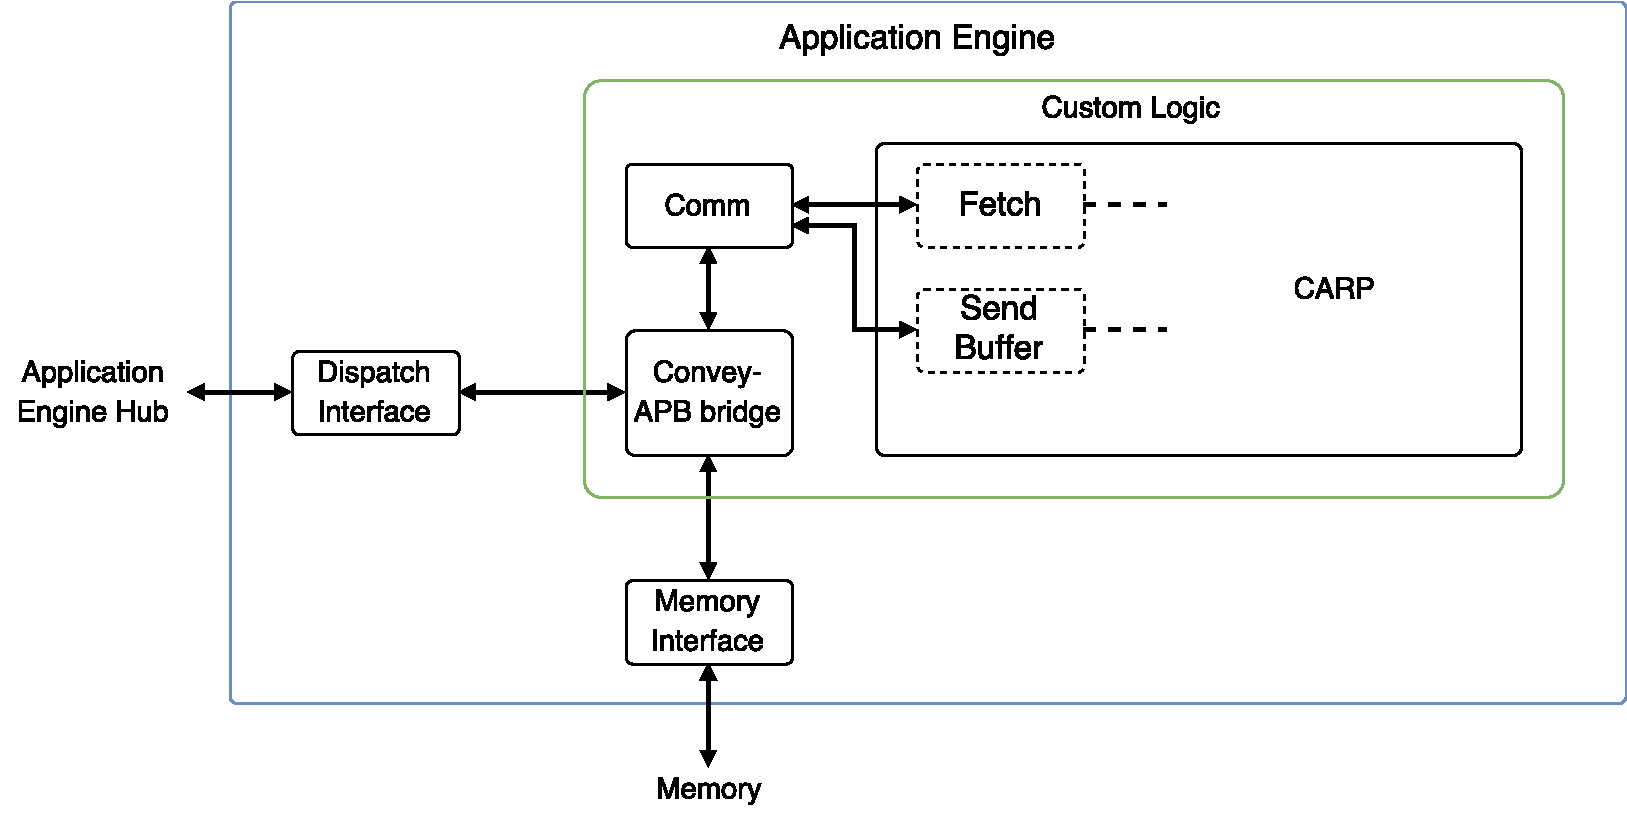
\includegraphics[width=\linewidth]{fig/convey-io-carp-overview}
  \caption{Implementation of the CARP platform within the AE architecture.}
  \label{fig:convey-io-carp-overivew}
\end{figure}

\begin{figure}[ht]
  \centering
  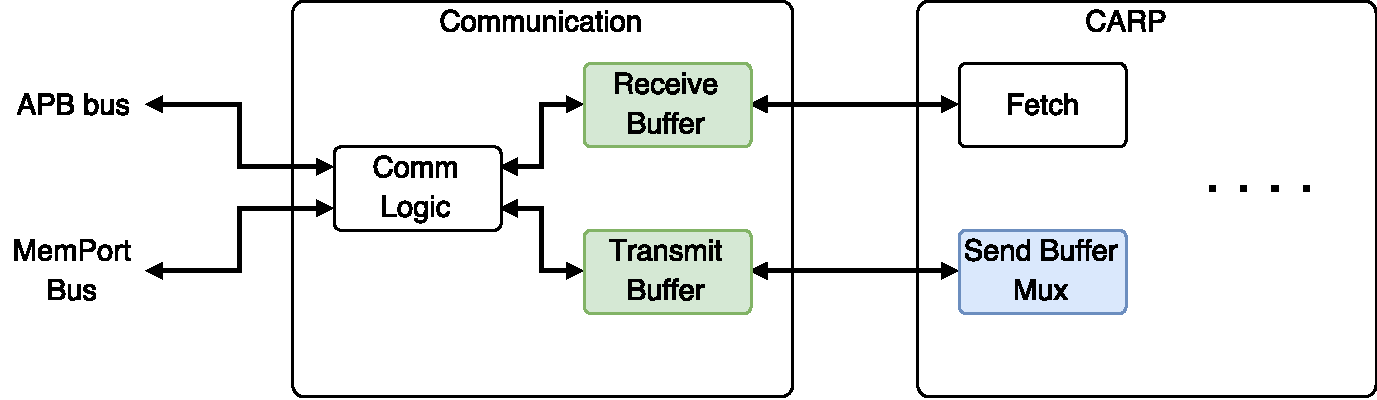
\includegraphics[width=0.8\linewidth]{fig/comm-io}
  \caption{
    The communication module interfaces with the CARP platform through two
    buffers, transmit and receive. Outwards, the communication module exposes two
    buses, an APB bus and a generic memory interface.
  }
  \label{fig:comm-io}
\end{figure}

To avoid having to rewrite the Fetch and Send Buffer Mux modules inside CARP,
the new communication module provides the same interface towards them as the old
one did; two data buffers, transmit and receive, buffer count signals and
read/write enable signals. Both data buffers are implemented as FIFO-queues with
counter registers and ready-valid access interfaces.

\begin{figure}[ht]
  \centering
  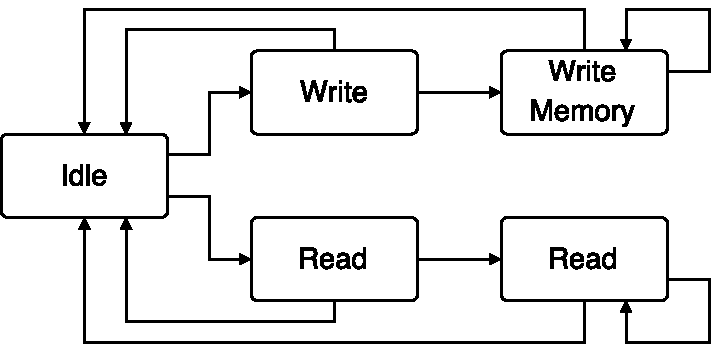
\includegraphics[width=0.5\linewidth]{fig/comm-fsm}
  \caption{State machine controlling the communication module.}
  \label{fig:comm-fsm}
\end{figure}

\figurename~\ref{fig:comm-fsm} shows the state machine controlling the operation
of the communication module. From the idle state, a transition to either the
Write or Read states can be triggered by asserting the PSEL signal on the APB
bus. Depending on wether or not the PWRITE signal is asserted, the state machine
will transition into the corresponding state. In this case, write refers to
writing data from the host to the receive buffer, and read refers to reading
data from the transmit buffer to the host. In the Write state, three bits in the
PADDR signal is used to further determine what is to happen. The possible
actions are as follows:

\begin{enumerate}
\item Write PWDATA to Receive Buffer. Transition to Idle state.
\item Set starting address register to PWDATA. Transition to Idle state.
\item Set end address register to PWDATA. Transition to Idle state.
\item Prepare to start transferring data from memory to Receive Buffer.
  Transition to Write Memory state.
\end{enumerate}

In the Write Memory state, read requests are generated on the MemPort bus and
received data is stored into the Receive Buffer. The Read and Read Memory states
have similar functionality, but writes data from the Transmit Buffer either
directly to the APB bus or to memory. In general, transfers of five 32-bit words
or less are done via the APB, while larger transfers go via memory. This is
however something that is specified in the SDK, not implemented in hardware.
That means that the system can be implemented to run on platforms without
on-board memory, as the MemPort interface can simply be tied off in that case.

The ConveyApbBridge-module serves, as the name implies, as a bridge between the
interfaces provided by the Convey PDK and the Communication module. The Dispatch
interface drives the APB bus, while the Memory Controller interface is wired
against the MemPort.

\clearpage

\section{Readout}
\label{sec:readout}

The Readout module extends the CARP platform with a reconfigurable Spiking
Neural Network operating in a data-driven fashion, synchronized to the clock of
state steps performed in the Cellular Automaton. Each layer of the network is
implemented as a stage in a pipeline. With every step of the CA, new input is
fed to the input layer and its output is fed as input to the next layer and so
on throughout the network. In other words, the number of state steps it takes
for data to propagate through the readout module as a whole is equal to the
number of layers in the network. The output from the final layer is routed back
into the CA. It is also stored in the Readout Buffer, from where it can be read
back to the host.

\begin{figure}[ht]
  \centering
  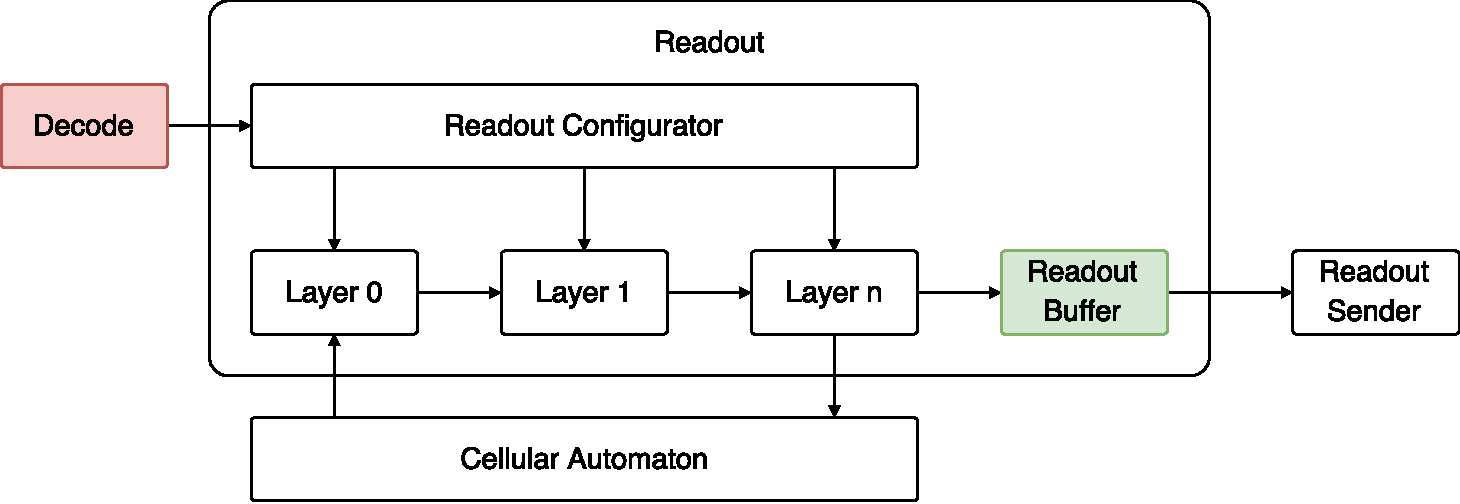
\includegraphics[width=\linewidth]{fig/readout-io}
  \caption{Logical overview of the Readout module.}
  \label{fig:readout-io}
\end{figure}

\figurename~\ref{fig:readout-io} shows, at a high level of abstraction, how the
Readout module is connected to the CARP system as whole. A subset of cell states
are routed out of the CA and into the Readout module as input to the first layer
of the network, the input layer. Within each layer, a number of neurons process
the input to the layer, as shown in \figurename~\ref{fig:readout-layer}. Based
on this input, they update their activation values, which again are fed to the
next layer to be used as input to those neurons in the next step.

\begin{figure}[ht]
  \centering
  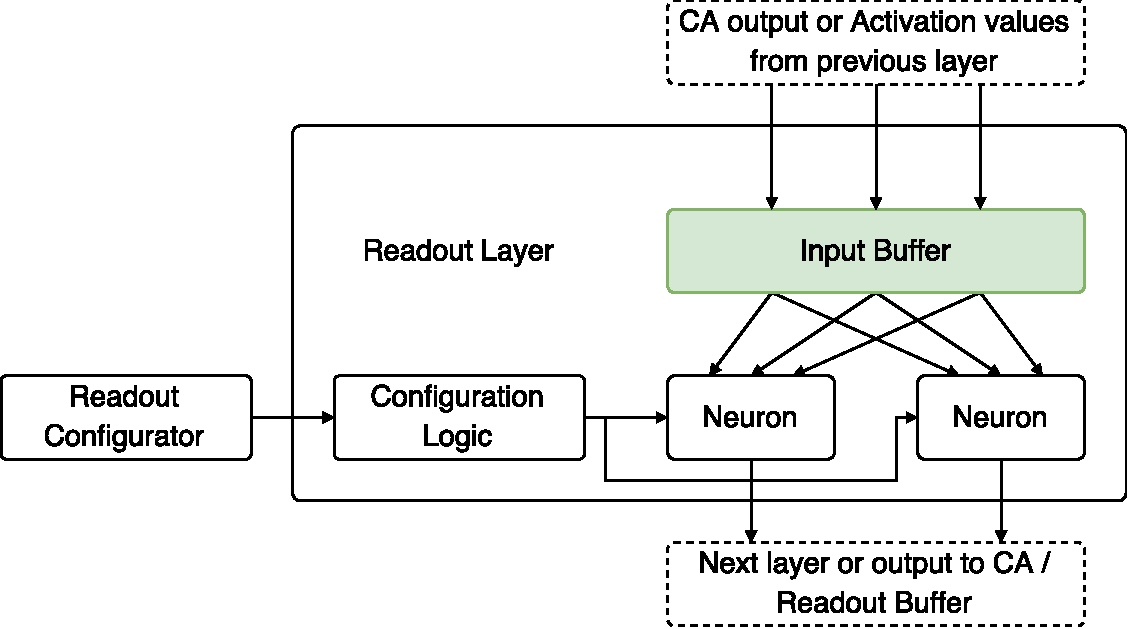
\includegraphics[width=0.8\linewidth]{fig/readout-layer}
  \caption{Logical overiew of one network layer in the Readout module.}
  \label{fig:readout-layer}
\end{figure}

The activation value of a neuron can be either 0 or 1, based on a very simple
calculation, as shown in \figurename~\ref{fig:readout-neuron}. For each of its
incoming edges, a neuron has a pair of registers, the edge weight and a counter.
The counter keeps track of how many spikes the neuron has received via the
corresponding edge, and the weight is a threshold, indicating how many spikes
must arrive via the edge before the neuron can fire. When all counters values
are equal to or greater than their weights, the neuron fires and the counters
are reset.

\begin{figure}[ht]
  \centering
  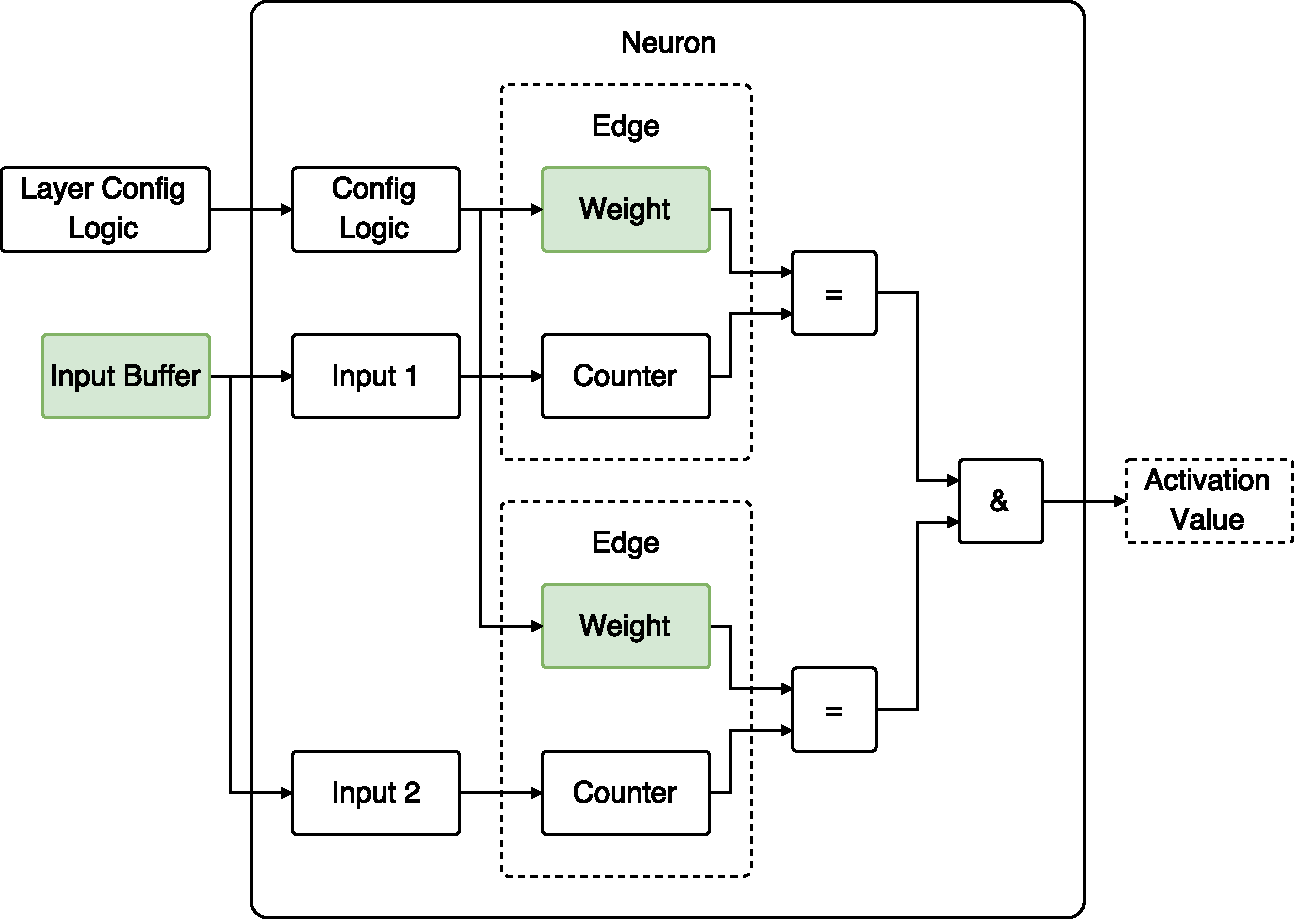
\includegraphics[width=0.8\linewidth]{fig/readout-neuron}
  \caption{Logical overview of a single neuron in the Readout module.}
  \label{fig:readout-neuron}
\end{figure}

To reduce the amount of resources required for the implementation, some
restrictions apply with regards to which network topologies are possible to
implement. All networks must be entirely feed-forward, that is they can not
contain any recurrent connections, the total number of neurons can not exceed
$2^{16}-1$ and the final layer must contain only a single neuron. The topology
of a network is given as a parameter to the module at synthesis time, and can
not be reconfigured while the system is running. It describes how many layers
the network consists of and how many neurons each of them consist of. Networks
are also implemented fully connected, all neurons in a layer are connected to
all neurons in the previous layer.

The module can be in one of two states, the default Processing state and the
Configuration state. In the Processing state, data flows through the network in
the manner described above. As mentioned, the topology of the network is defined
at synthesis time. The weights however, can be reconfigured while the system is
running. This allows for rapid exploration of networks with different
characteristics. The transition to the Configuration state is triggered when the
Readout module receives a WriteWeight instruction from the Decode module.
Accompanying the instruction is payload consisting of a 16-bit address and an
8-bit weight value. \figurename~\ref{fig:readout-addressing-scheme} shows an
example of how edges and their corresponding weight registers are addressed,
starting from address 0 in the top left, increasing top to bottom between the CA
output and the first layer, then continuing from the top in the next.

A WeightWrite instruction completes the same clock cycle it is received,
returning the module to the Processing state in the subsequent cycle. This is
done by wiring the weight bus directly into each neuron and decoding the address
value using entirely combinatorial logic to decide which weight should be
updated. At the top level, the address is used to decide into which layer the
weight should be written. That layer then receives a high write enable signal
and the address of the weight within the layer. Similarily, the targeted layer,
uses this address to find the neuron to which the targeted weight belongs and
passes the write enable signal into it along with the address of the weight
within that neuron. The neuron asserts write enable for the targeted register
which will then contain the new weight value the subsequent clock cycle.

\begin{figure}[ht]
  \centering
  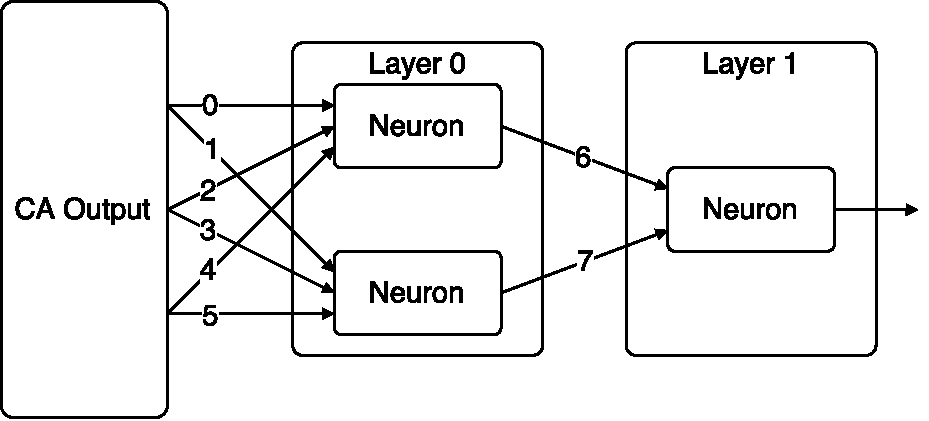
\includegraphics[width=0.6\linewidth]{fig/readout-addressing-scheme}
  \caption{Example of how edges/weights are addressed counting from left to right, top to bottom.}
  \label{fig:readout-addressing-scheme}
\end{figure}

With the configuration in \figurename~\ref{fig:readout-addressing-scheme} as an
example; a WriteWeight instruction arrives with the address 7 in the payload. At
the top level, the module knows that addresses in the range $\lbrack 6, 7 \rbrack$ belong to
Layer 1. The address of the targeted weight within that layer is found by
subtracting the total number edges between all previous layers from the global
address, i.e. $7 - 6 = 1$. Inside that layer, the correct neuron is found by
utilizing the fully connected nature and calculating $Addr \bdiv NeuronsPrevious
Layer$. The address of the weight within that neuron is calculated with $Addr
\bmod NeuronsPreviousLayer$. In this example, the only neuron in the layer
receives the weight address 1 and updates the correct weight accordingly.

\clearpage

\section{Cellular Automaton}
\label{sec:cellular-automaton}

Alongside the Development and Readout modules, the Cellular Automaton module forms
the core of the CARP system. It is responsible for simulating the dynamic
behavior of and interaction between cells. The CA module has been partially
ported to Scala and modified to support routing live cell states out of the
SBlock Matrix and feedback from the Readout Module back in. To achieve this, the
top-level logic responsible for orchestrating configuration of the SBlock Matrix
and the matrix itself have been reimplemented from scratch in Chisel, while the
Live Count related modules remain unchanged and are still implemented in VHDL.

\begin{figure}[ht]
  \centering
  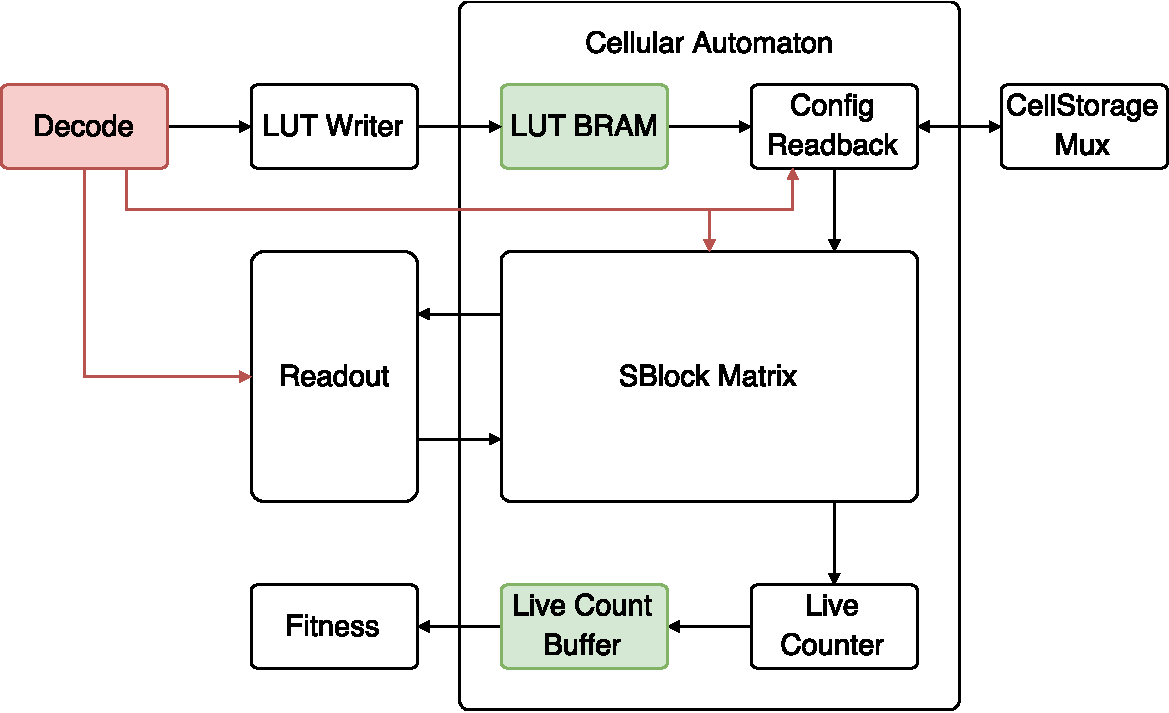
\includegraphics[width=0.8\linewidth]{fig/ca-io}
  \caption{The Cellular Automaton module and surrounding modules.}
  \label{fig:ca-io}
\end{figure}

As shown in \figurename~\ref{fig:ca-io}, the central part of the CA module is
the SBlock Matrix, a 2D/3D matrix of modules connected in a regular grid. The
modules can be either an SBlock or a FeedbackCell. An SBlock uses the states of
the the cells in its von Neumann neighborhood as input to a configurable
Look-Up-Table (LUT) and updates its own state, stored in a Flip-flop (FF), with
the output from the LUT. A FeedbackCell on the other hand, receives only the
output from the Readout module as input and updates its state with this value.
Both are shown in \figurename~\ref{fig:ca-celltypes}. State updates happen
synchronously throughout the matrix, all cells march in step so to speak. At
synthesis time, the SBlock Matrix utilizes two lists of coordinates, one
indicating which cells should be FeebackCells, and one indicating which cells'
states should be routed out of the module to be wired as input to the Readout
module. All cells not in the FeedbackCells list will be instantiated as SBlocks.

\begin{figure}[ht]
  \subfloat[SBlock \label{fig:sblock}]{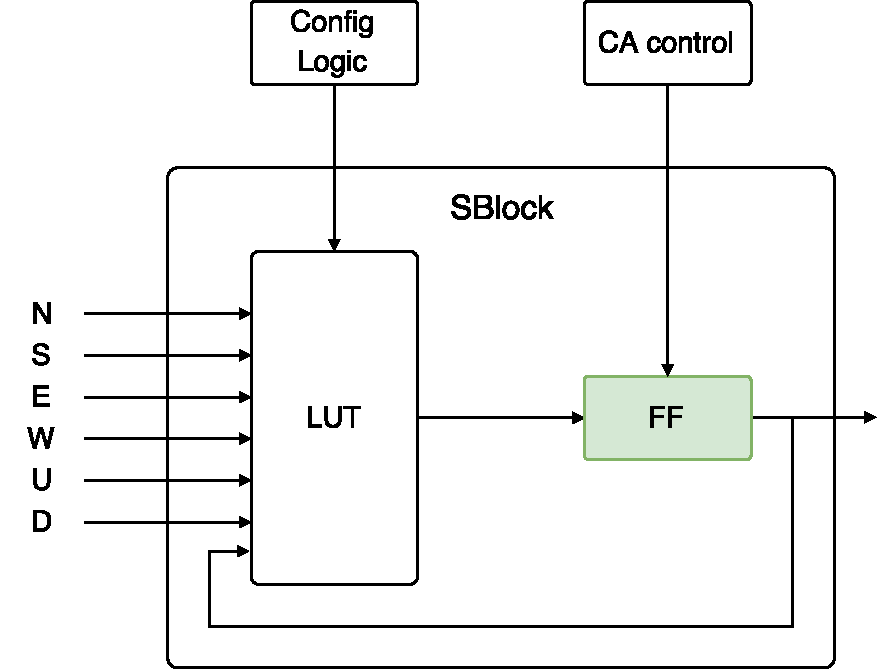
\includegraphics[width=0.45\linewidth]{fig/sblock}}
  \qquad
  \subfloat[FeedbackCell \label{fig:feedbackcell}]{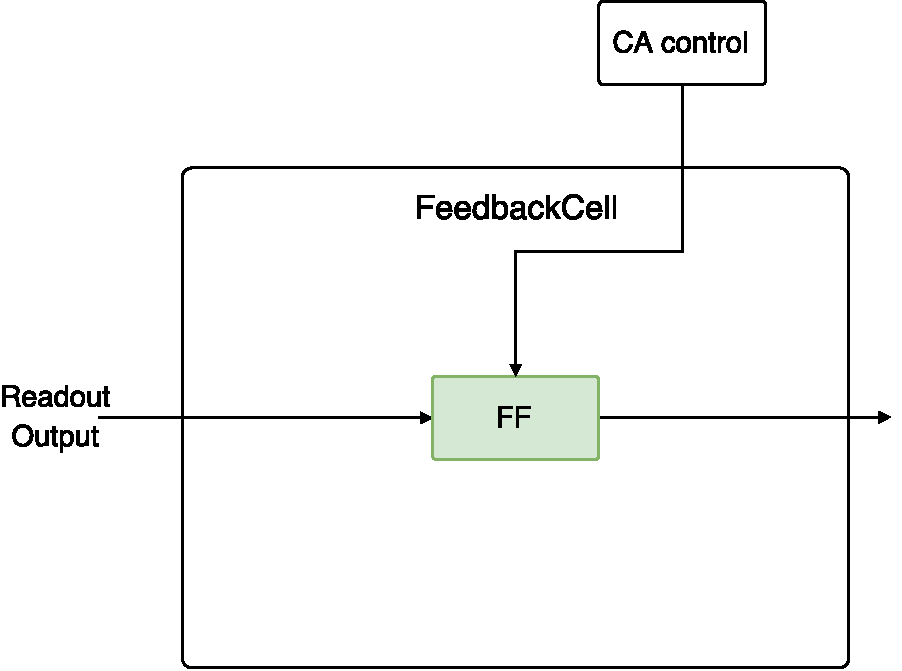
\includegraphics[width=0.45\linewidth]{fig/feedbackcell}}
  \caption{
    Detailed view of the SBlock and FeedbackCell modules used in the
    SBlock Matrix.\label{fig:ca-celltypes}
  }
\end{figure}

The state machine in \figurename~\ref{fig:ca-fsm} controls the operation of the
CA module. Starting from the Idle state, the module can transition into one of
three states based on instructions received from the Decode module. In the
Configuration state, the SBlocks in the SBlock Matrix are configured one row at
a time. LUTs are configured with different values depending on the cell type of
the cell the SBlock simulates. FeedbackCells are not configurable and can not
develop into a different cell type, so they are simply ignored with regards to
LUT configuration. The state of each cell is also read from Cell Storage and
configured into FFs.

In the Readback state, the state of each cell is read back to the Cell Storage.
Similar to configuration, this happens row by row.

The Step state is the core functionality of the CA module. Here, all
cells/SBlocks synchronously update their states. The instruction also includes a
16-bit number in its payload, indicating how many steps to perform in bulk. When
a step has completed, a signal is sent to the Readout module indicating that it
should perform one step of its pipeline, and start processing the new cell
states it has received.

\begin{figure}[ht]
  \centering
  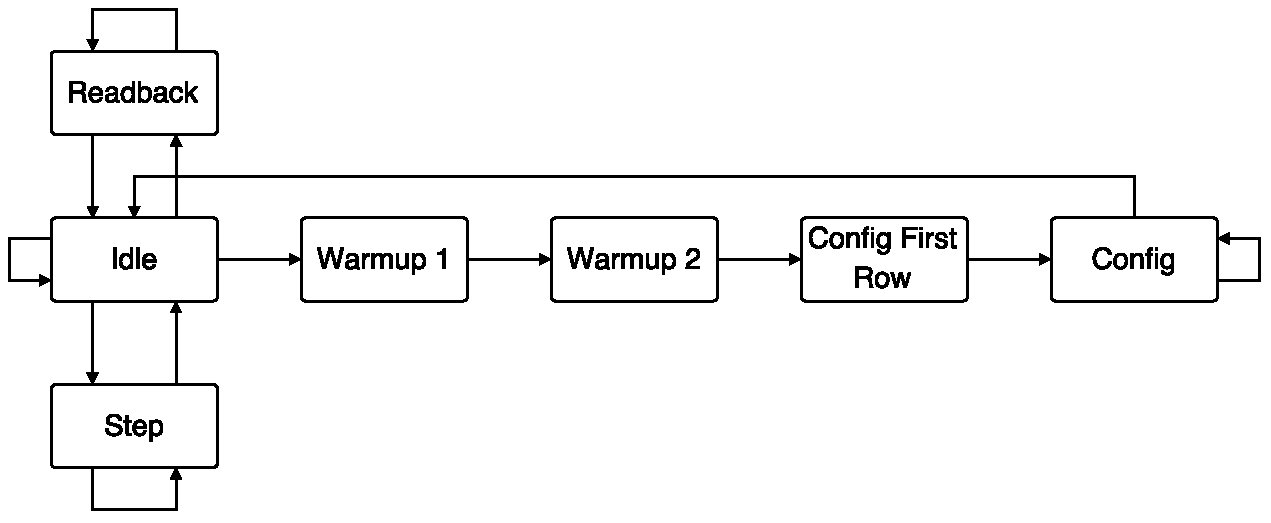
\includegraphics[width=0.8\linewidth]{fig/ca-fsm}
  \caption{State machine controlling the operation of the CA module.}
  \label{fig:ca-fsm}
\end{figure}

While the Live Count and Fourier Transform modules implemented by Lundal have
not been used in the work presented in this thesis, they have been left
unchanged and functional for possible future use.

\clearpage

\section{Miscelaneous Modules}
\label{sec:misc-modules}

In addition to the major additions and changes to the system outlined in the
previous sections, several smaller changes have been made throughout the system
to accomodate the new functionality.

\subsection{Readout Sender}

The Readout Sender is a small module added to facilitate transferring Readout
output data from the Readout Buffer to the host. It receives instructions from
the Decode module and places data in the Transfer Buffer of the Communication
module via the Send Buffer Mux. A single ReadReadout instruction causes 32 words
to be transferred.

\begin{figure}[ht]
  \centering
  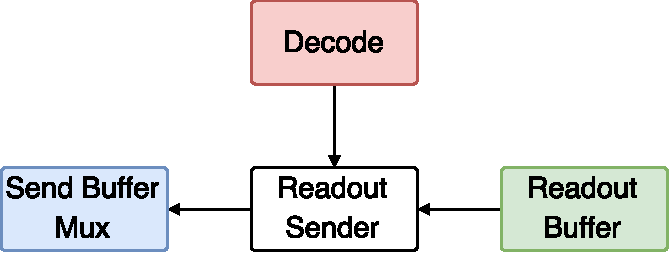
\includegraphics[width=0.6\linewidth]{fig/readout-sender}
  \caption{Readout Sender }
  \label{fig:ca-fsm}
\end{figure}

\subsection{Decode}

The Decode module is responsible for parsing instructions, setting control
signals and passing instruction parameters to modules. It has been extended to
support the two new instructions. For the ReadReadout instruction, it signals the
Readout Sender to initialize a transfer, as well as setting the necessary
control signals to the Send Buffer Mux to allow data from the Readout Sender to
pass through to the Transfer Buffer. In the case of a WriteWeight instruction,
the address and weight value parameters are extracted from the instruction
payload passed on to the Readout module along with the control signals
indicating that a weight should be updated.

\subsection{Information Sender}

Parameterization has been used extensively throughout the CARP hardware system
to allow for as much flexibility as possible. To avoid having to update the
software API every time the system is synthesized with new parameters, Lundal
introduced the Information Sender, a module that allows the API to query the
hardware for information. When a ReadInformation instruction is issued, it
places a number of system parameters into Transfer Buffer; CA size, wether or
not wrapping is enabled, number of bits per cell state and type, control flow
counter sizes, maximum number of development rules and information about the
fitness module. The module has been extended to also include information
relating to the Readout module. The added parameters are; number of network
layers in the Readout topology, number of output cells from the CA, and the
number of neurons in each network layer. Since the system can be synthesized
with any number of network layers, the total size of the payload generated by
the Information Sender will depend on this number.
\clearpage

\section{Parameterization}
\label{sec:parameterization}

Many aspects of the CARP hardware platform are parameterized. With the
introduction of the Readout module, a few new parameters have been added.
Readout Buffer size, Readout Weight bits and Readout Address Bits are integer
values controlling bus widths and buffer sizes. The CA Output Cells and CA
Feedback Cells parameters are lists of (x, y, z) coordinate triplets indicating
the location of output and Feedback cells respectively. The Readout Topology
parameter determines the number of network layers and number of neurons in each.
For instance, Readout Topology value of $(10, 5, 3, 2, 1)$ will result in a 5
layer network with 10 neurons in layer 0, 5 in layer 1, 3 in layer 2, 2 in layer
3 and 1 neuron in the output layer. A full list of parameters is given in
Table~\ref{tbl:parameters}.

To leverage the strengths of Chisel and the Object-Oriented aspects of the
underlying Scala, parameters have been organized into an interface (or trait in
Scala jargon), \texttt{CarpParameters}. This allows for more flexibility in
expressing the more complicated parameters such as CA Output Cells and CA
Feedback Cells.

\renewcommand{\arraystretch}{1.2}
\begin{table}[ht]
    \begin{tabular}{l|c|l}
    Parameter                 & Values      & Note                             \\ \hline
    Tx/Rx Buffer Address Bits & [1, $\infty$]    & Determines size of Rx/Tx Buffers \\
    ProgramCounter Bits       & [1, 16]     & Restricted by ISA/Decode         \\
    Matrix Width              & [2, 256]    & Restricted by ISA/Decode         \\
    Matrix Height             & [2, 256]    & Restricted by ISA/Decode         \\
    Matrix Depth              & [1, 256]    & Restricted by ISA/Decode         \\
    Matrix Wrap               & True, False & ~                                \\
    Cell Type Bits            & [1, 32]     & Restricted by ISA/Decode         \\
    Jump Counter Amount       & [1, 256]    & Restricted by ISA/Fetch          \\
    Jump Counter Bits         & [1, 32]     & Restricted by ISA/Fetch          \\
    LUT Configuration Bits    & 1, 2, 4, 8  & Restricted by SBlocks            \\
    Rule Amount               & [1, $\infty$]    & ~                                \\
    Rules Tested in Parallell & [1, $\infty$]    & ~                                \\
    Rule Vector Buffer Size   & [1, $\infty$]    & ~                                \\
    Fitness Buffer Size       & [1, $\infty$]    & ~                                \\
    Readout Buffer Size       & [1, $\infty$]    & ~                                \\
    Readout Weight Bits       & [1,  8]     & Restricted by ISA/Decode         \\
    Readout Address Bits      & [1, 16]     & Restricted by ISA/Decode         \\
    Readout Topology          & N/A         & List of positive integers                  \\
    CA Output Cells           & N/A         & List of (x, y, z) coordinates    \\
    CA Feedback Cells         & N/A         & List of (x, y, z) coordinates    \\
    \end{tabular}
    \caption{List of parameters for the CARP hardware}
    \label{tbl:parameters}
\end{table}

\renewcommand{\arraystretch}{1}
\clearpage

\section{Software API}

\cleardoublepage
%%% Local Variables:
%%% mode: latex
%%% TeX-master: "../thesis"
%%% End:
